\documentclass[a4paper,9pt]{extarticle}

%=========================================================
% PACKAGES
%=========================================================

\usepackage[
a4paper,
top=1.8cm,
bottom=1.5cm,
footskip=7mm,
left=1cm,
right=1cm,
headheight=14pt,
headsep=5mm
]{geometry}
\usepackage[T1]{fontenc}
\usepackage[utf8]{inputenc}
\usepackage[french]{babel}

\usepackage[sfdefault]{FiraSans}
\renewcommand{\familydefault}{\sfdefault}

\usepackage{multicol}
\setlength{\columnsep}{0.7cm}

\usepackage{amsmath,amssymb}

\usepackage{titlesec}
\usepackage{enumitem}

\usepackage{tcolorbox}
\tcbuselibrary{skins,breakable}

\usepackage{xcolor}

\usepackage{graphicx}
\usepackage{float}

\usepackage{tikz}

\usepackage{fancyhdr}
\usepackage[hidelinks]{hyperref}


%=========================================================
% PAGE SETTINGS
%=========================================================

\setlength{\parindent}{0pt}
\setlength{\parskip}{1.5pt}

\setlength{\abovedisplayskip}{4pt}
\setlength{\belowdisplayskip}{4pt}

\setlist[itemize]{
leftmargin=*,
itemsep=1pt,
topsep=1pt
}


%=========================================================
% COLORS
%=========================================================

\definecolor{Blue}{HTML}{E3F0FF}
\definecolor{Green}{HTML}{E3F7EA}
\definecolor{Pink}{HTML}{FFE5ED}
\definecolor{Orange}{HTML}{FFF0DC}
\definecolor{Purple}{HTML}{EEE7FF}
\definecolor{Yellow}{HTML}{FFFADB}


\definecolor{BlueTitle}{HTML}{285B8F}
\definecolor{GreenTitle}{HTML}{287052}
\definecolor{PinkTitle}{HTML}{A84063}
\definecolor{OrangeTitle}{HTML}{A96500}
\definecolor{PurpleTitle}{HTML}{6245A5}


%=========================================================
% HEADER
%=========================================================

\pagestyle{fancy}

\fancyhf{}

\fancyhead[L]{\small\textbf{Game Theory and Strategic Decisions}}
\fancyhead[C]{\small Revenue Equivalence, Reserve Prices and eBay}
\fancyhead[R]{\small Week 09 --- 09-15/11/2026}

\fancyfoot[C]{\small\href{https://github.com/AlphaXT38G/notes_ba5}{github.com/AlphaXT38G/notes\_ba5}}
\fancyfoot[R]{\small \thepage}

\renewcommand{\headrulewidth}{0.4pt}



%=========================================================
% TITLES
%=========================================================

\titleformat{\section}
{\large\bfseries\color{BlueTitle}}
{}{0pt}{}

\titlespacing{\section}
{0pt}{6pt}{3pt}


% separator

\newcommand{\separator}{
\vspace{2pt}
\hrule
\vspace{3pt}
}


%=========================================================
% BOXES
%=========================================================

% Boxes are kept whole (unbreakable): inside multicols, a box split by tcolorbox
% leaves an empty column behind it.

% DEFINITION - blue
\newtcolorbox{definition}{
enhanced,
unbreakable,
colback=Blue,
colframe=BlueTitle,
boxrule=0.7pt,
arc=0mm,
title=\textbf{Definition},
fonttitle=\bfseries
}

% IMPORTANT - pink
\newtcolorbox{important}{
enhanced,
unbreakable,
colback=Pink,
colframe=PinkTitle,
boxrule=0.7pt,
arc=0mm,
title=\textbf{Key idea},
fonttitle=\bfseries
}

% FORMULAS - green
\newtcolorbox{formula}{
enhanced,
unbreakable,
colback=Green,
colframe=GreenTitle,
boxrule=0.7pt,
arc=0mm,
title=\textbf{Key formulas},
fonttitle=\bfseries
}

% WARNING - orange
\newtcolorbox{warning}{
enhanced,
unbreakable,
colback=Orange,
colframe=OrangeTitle,
boxrule=0.7pt,
arc=0mm,
title=\textbf{Warning},
fonttitle=\bfseries
}

% EXAMPLE - purple
\newtcolorbox{example}{
enhanced,
unbreakable,
colback=Purple,
colframe=PurpleTitle,
boxrule=0.7pt,
arc=0mm,
title=\textbf{Example},
fonttitle=\bfseries
}

% SUMMARY - orange
\newtcolorbox{summary}{
enhanced,
unbreakable,
colback=Yellow,
colframe=OrangeTitle,
boxrule=0.7pt,
arc=0mm,
title=\textbf{Summary},
fonttitle=\bfseries
}



%=========================================================
% FIGURE BOX
%=========================================================

\newtcolorbox{figurebox}{
enhanced,
colback=white,
colframe=gray,
boxrule=0.5pt,
arc=0mm,
center
}



%=========================================================
% DOCUMENT
%=========================================================

\begin{document}

%\footnotesize   --> To reduce the size of the text

\thispagestyle{fancy}



\begin{multicols}{2}



%=========================================================
\section{Last Lecture: Private-Value Auctions}


No uncertainty about the object; each player has a \textbf{private, independent valuation
$v_i$}.


\begin{itemize}

\item \textbf{First-price}: values i.i.d.\ uniform on $[0,1]$ $\rightarrow$
$b_i = \frac{N-1}{N} v_i$. More information about the others may change my bid.

\item \textbf{Second-price}: $b_i = v_i$ is dominant; no information about the others should
change it.

\end{itemize}



%=========================================================
\section{Today's Agenda}


\begin{itemize}

\item \textbf{Revenue equivalence theorem}: first-, second-, third-price and all-pay auctions
all yield the same expected revenue.

\item \textbf{Reserve prices}: not the same revenue; there is a reserve price that maximizes
it.

\item \textbf{eBay}: proxy bidding, private vs common value, sniping, reserve prices, winner's
curse and reputation.

\end{itemize}



%=========================================================
\section{Revenue Equivalence Theorem}


\begin{definition}

\textbf{REVENUE EQUIVALENCE THEOREM}

$N$ bidders, each with an \textbf{independent private valuation} drawn from a distribution
$F$. Any two auction mechanisms in which

\begin{itemize}

\item in equilibrium, given $v_1, \ldots, v_N$, \textbf{the good is allocated the same way},
and

\item any bidder with valuation 0 has an expected utility of 0,

\end{itemize}

yield the \textbf{same expected revenue} for the auctioneer, and each player with value $v$
makes the \textbf{same expected payment} $\chi(v)$.

\end{definition}


\begin{important}

\textbf{How to use it}: compute $\chi(v)$ in the second-price auction; write the expected
payment of the new format as a function of the bid; set them equal and solve for the bid.

\end{important}



%=========================================================
\section{Second-Price Auctions}


Bidding one's value is dominant. Uniform on $[0,V]$, $k$-th statistic of $n$ draws:
$\mathcal{S}_k = \frac{n+1-k}{n+1} V$. The winner (value $v$) pays the highest of the other
$N-1$ values, on average $\frac{N-1}{N} v$.


\begin{formula}

Expected payment = (Prob.\ $v$ is the highest) $\times$ (payment if winning):

\[
\text{Expected Payment}(v) = v^{N-1}\,\frac{N-1}{N}\, v
\]

($v$ uniform on $[0,1]$; each of the $N-1$ others is below $v$ with prob.\ $v$).

\end{formula}



%=========================================================
\section{First-Price Auctions}


If others bid $b_j = a v_j$: $\max_b\, (v - b)\left(\frac{b}{a}\right)^{N-1}$ gives
$b = \frac{N-1}{N} v$ (last lecture).


\begin{formula}

\textbf{Alternatively}, by revenue equivalence:

\[
\text{Expected Payment}(v_i) = v_i^{N-1}\,b(v_i) = v_i^{N-1}\frac{N-1}{N} v_i
\]

$v_i^{N-1}$ is the probability of winning (same strategy for all), so

\[
b(v_i) = \frac{N-1}{N}\, v_i
\]

\end{formula}



%=========================================================
\section{Third-Price Auctions}


\begin{warning}

Bidding truthfully is \textbf{not} dominant: player $i$ bids $v_i$, another wins with
$b^{(1)} > v_i$ and pays $b^{(2)} < v_i$. Bidding above $b^{(1)}$ she would have won and paid
$b^{(2)} < v_i$.

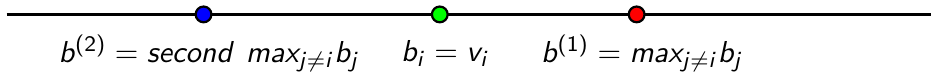
\includegraphics[width=\linewidth]{../images/week09_01.png}

\end{warning}


\begin{formula}

Guess $b(v) = a v$ (the highest value wins $\rightarrow$ the theorem applies).

\begin{itemize}

\item If $v_i$ is the highest, $i$ pays $a \times v^{(3)}$; $v^{(3)}$ is the 2nd highest of
the $N-1$ others, uniform on $[0, v_i]$:

\[
E[v^{(3)}] = \frac{N-2}{N}\, v_i
\]

\item $\text{Expected Payment}(v_i) = v_i^{N-1}\, a\, \frac{N-2}{N}\, v_i$

\end{itemize}

Same as first/second-price if $a = \frac{N-1}{N-2}$:

\[
b(v_i) = \frac{N-1}{N-2}\, v_i
\]

\end{formula}


\begin{important}

\textbf{Overbidding}: $b(v_i) > v_i$. You pay only the third bid when you win, so bidding
above your value rarely costs you more than your value. (Same result by maximizing.)
E.g.\ (not on the slides) $N = 3$: $b = 2v$.

\end{important}



%=========================================================
\section{All-Pay Auction}


\begin{itemize}

\item Each bidder submits a sealed bid; the highest bid wins.

\item \textbf{Each bidder pays} his own bid to the seller.

\item Suppose the highest-valuation bidder wins; use the theorem to get the bid; ex-post
verify that the highest value indeed wins.

\end{itemize}


\begin{formula}

Uniform on $[0,1]$. A bidder with value $v_i$ wins with probability $v_i^{N-1}$ and pays
$b(v_i)$ \textbf{whether he wins or not}. First-price expected payment:

\[
v_i^{N-1}\frac{N-1}{N} v_i = \frac{N-1}{N} v_i^N
\]

so

\[
b(v_i) = \frac{N-1}{N}\, v_i^N
\]

\end{formula}


(Not on the slides) $b$ increases with $v$, so the highest value wins: verified. With 2
bidders, $b = v^2/2$. Seller's expected revenue in all four formats:
$N\int_0^1 \frac{N-1}{N}v^N dv = \frac{N-1}{N+1}$ ($1/3$ for 2 bidders).



%=========================================================
\section{Auctions with a Reserve Price}


\begin{definition}

\textbf{RESERVE PRICE}: a price below which the seller is not willing to sell.

Second-price with reserve $R$: the highest bidder gets the item if bid $\ge R$, and pays
\textbf{the largest of the second-highest bid and $R$}.

\begin{itemize}

\item Bids 0.3 and 0.6, $R = 0.4$: pays 0.4.

\item Bids 0.5 and 0.6, $R = 0.4$: pays 0.5.

\item Bids 0.3 and 0.36, $R = 0.4$: nobody wins.

\end{itemize}

\end{definition}


\begin{warning}

\textbf{Not the same expected revenue} as without reserve: in the 3rd example the
\textbf{allocation is different}.

\end{warning}



%=========================================================
\section{Second-Price with Reserve Price}


2 bidders, uniform on $[0,1]$. Treat $R$ as \textbf{another bidder whose bid we know}.
Dominant: bid own value if $v > R$; don't bid if $v \le R$.


\begin{center}

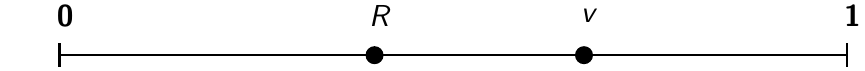
\includegraphics[
width=0.9\linewidth
]{../images/week09_02.png}

\end{center}


A bidder with $v > R$: wins with prob.\ $v$; if winning, the other is below $R$ with prob.\
$R/v$ (pays $R$), otherwise uniform on $[R, v]$ (pays $\frac{v+R}{2}$ on average).


\begin{formula}

\[
\frac{R}{v}R + \left(1 - \frac{R}{v}\right)\frac{v+R}{2} = R + \frac{(v-R)^2}{2v}
\]

\[
\text{Expected Payment}(v > R) = v\left(R + \frac{(v-R)^2}{2v}\right)
\]

\end{formula}



%=========================================================
\section{First-Price with Reserve Price}


A bidder with $v > R$ always bids above $R$. Same allocation as the second-price auction with
the same $R$ $\rightarrow$ \textbf{revenue equivalence applies}.


\begin{formula}

Does not bid if $v \le R$; if $v > R$:

\[
b(v) = R + \frac{(v-R)^2}{2v}
\]

\end{formula}


(Check: $R = 0$ gives back $b = v/2$.)



%=========================================================
\section{Optimal Reserve Price}


Second-price, 2 bidders, $U[0,1]$: compare the revenue when the reserve goes from $R$ to
$R + \epsilon$, over all $v_l < v_h$.


\begin{center}

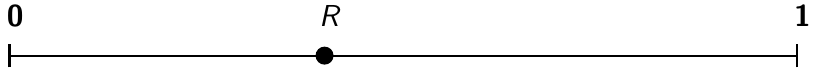
\includegraphics[
width=0.9\linewidth
]{../images/week09_03.png}

\end{center}


\begin{itemize}

\item $v_l < v_h < R$: no impact.

\item $R + \epsilon < v_l < v_h$: no impact.

\item $v_l < R < R + \epsilon < v_h$: revenue $+\epsilon$ (prob.\ $2R(1-R)$).

\item $v_l < R < v_h < R + \epsilon$: revenue $-R$ (prob.\ $2\epsilon R$).

\item $R < v_l < R + \epsilon < v_h$: $+\sim\epsilon$ (prob.\ $2\epsilon(1-R)$), order
$\epsilon^2$.

\end{itemize}


\begin{formula}

\[
\Delta\text{Revenue} = 2R(1-R)\epsilon - 2\epsilon R^2
\]

Zero at the optimum: $R^* = \frac{1}{2}$.

\end{formula}


(Not on the slides) Revenue with $R = 1/2$: $5/12 \approx 0.417 > 1/3$.



%=========================================================
\section{eBay}


Founded by Pierre Omidyar in 1995; over 1 billion active listings; over 180 million active
buyers; about 2 billion daily transactions; second online marketplace after Amazon.


\textbf{Listings}: description and pictures; ID and rating of the seller; current bid and
number of bids; minimum bid (a reserve price) \emph{and} whether there is a secret reserve
price; minimum increment; time left.


\begin{definition}

\textbf{PROXY BIDDING}

You enter the \textbf{maximum} you are willing to pay; eBay bids for you just enough to keep
you the high bidder.

\begin{itemize}

\item Minimum bid \$10, increment \$0.50. A enters \$25: current bid \$10.

\item B enters \$13: A's current bid rises to \$13.50.

\item C enters \$26: A is no longer the high bidder, notified by email.

\end{itemize}

The high bidder pays \textbf{the second-highest proxy bid plus the increment}.

\end{definition}


\begin{important}

\textbf{eBay's format $\approx$ second-price auction}. Unlike sealed bids, bidders see the
high bid evolve; unlike an English auction, they don't see all bids nor when others drop out.

\end{important}






\end{multicols}


\end{document}
